
%%%%%%%%%%%%%%%%%%%%%%%%%%%%%%%%%%%%%%%%%%%%%%%%%%%%%%%%%%%%%%%%%%%%%%%%%%%%%%%%%%%%%%%
%%%%%%%%%%%%%%%%%%%%%%%%%%%%%%%%%%%%%%%%%%%%%%%%%%%%%%%%%%%%%%%%%%%%%%%%%%%%%%%%%%%%%%%
% 
% This top part of the document is called the 'preamble'.  Modify it with caution!
%
% The real document starts below where it says 'The main document starts here'.

\documentclass[12pt]{article}

\usepackage{amssymb,amsmath,amsthm}
\usepackage[top=1in, bottom=1in, left=1.25in, right=1.25in]{geometry}
\usepackage{fancyhdr}
\usepackage{enumerate}
\usepackage{listings}
\usepackage{graphicx}
\usepackage{float}
\usepackage{multicol}
% Comment the following line to use TeX's default font of Computer Modern.
\usepackage{times,txfonts}
\usepackage{mwe}
\usepackage{caption}
\usepackage{subcaption}

\usepackage{tikz}
\def\checkmark{\tikz\fill[scale=0.4](0,.35) -- (.25,0) -- (1,.7) -- (.25,.15) -- cycle;} 



\makeatletter
\renewcommand*\env@matrix[1][*\c@MaxMatrixCols c]{%
  \hskip -\arraycolsep
  \let\@ifnextchar\new@ifnextchar
  \array{#1}}
\makeatother

\newtheoremstyle{homework}% name of the style to be used
  {18pt}% measure of space to leave above the theorem. E.g.: 3pt
  {12pt}% measure of space to leave below the theorem. E.g.: 3pt
  {}% name of font to use in the body of the theorem
  {}% measure of space to indent
  {\bfseries}% name of head font
  {:}% punctuation between head and body
  {2ex}% space after theorem head; " " = normal interword space
  {}% Manually specify head
\theoremstyle{homework} 

% Set up an Exercise environment and a Solution label.
\newtheorem*{exercisecore}{Exercise \@currentlabel}
\newenvironment{exercise}[1]
{\def\@currentlabel{#1}\exercisecore}
{\endexercisecore}

\newcommand{\localhead}[1]{\par\smallskip\noindent\textbf{#1}\nobreak\\}%
\newcommand\solution{\localhead{Solution:}}

%%%%%%%%%%%%%%%%%%%%%%%%%%%%%%%%%%%%%%%%%%%%%%%%%%%%%%%%%%%%%%%%%%%%%%%%
%
% Stuff for getting the name/document date/title across the header
\makeatletter
\RequirePackage{fancyhdr}
\pagestyle{fancy}
\fancyfoot[C]{\ifnum \value{page} > 1\relax\thepage\fi}
\fancyhead[L]{\ifx\@doclabel\@empty\else\@doclabel\fi}
\fancyhead[C]{\ifx\@docdate\@empty\else\@docdate\fi}
\fancyhead[R]{\ifx\@docauthor\@empty\else\@docauthor\fi}
\headheight 15pt

\def\doclabel#1{\gdef\@doclabel{#1}}
\doclabel{Use {\tt\textbackslash doclabel\{MY LABEL\}}.}
\def\docdate#1{\gdef\@docdate{#1}}
\docdate{Use {\tt\textbackslash docdate\{MY DATE\}}.}
\def\docauthor#1{\gdef\@docauthor{#1}}
\docauthor{Use {\tt\textbackslash docauthor\{MY NAME\}}.}
\makeatother

% Shortcuts for blackboard bold number sets (reals, integers, etc.)
\newcommand{\Reals}{\ensuremath{\mathbb R}}
\newcommand{\Nats}{\ensuremath{\mathbb N}}
\newcommand{\Ints}{\ensuremath{\mathbb Z}}
\newcommand{\Rats}{\ensuremath{\mathbb Q}}
\newcommand{\Cplx}{\ensuremath{\mathbb C}}
%% Some equivalents that some people may prefer.
\let\RR\Reals
\let\NN\Nats
\let\II\Ints
\let\CC\Cplx

%\textbf{Code:}
%\begin{center}
%  \lstinputlisting{NewtonsMethodP5.m}
%\end{center}
%
%\textbf{Console:}
%\begin{center}
%  \lstinputlisting{P5C.txt}
%\end{center}
%\vspace{.15in}


%\begin{figure}[H]
%  \begin{center}
%    \caption{The one-norm unit ball}
%    \includegraphics[width=.76\textwidth]{1norm.png}
%  \end{center}
%\end{figure}




%%%%%%%%%%%%%%%%%%%%%%%%%%%%%%%%%%%%%%%%%%%%%%%%%%%%%%%%%%%%%%%%%%%%%%%%%%%%%%%%%%%%%%%
%%%%%%%%%%%%%%%%%%%%%%%%%%%%%%%%%%%%%%%%%%%%%%%%%%%%%%%%%%%%%%%%%%%%%%%%%%%%%%%%%%%%%%%
% 
% The main document start here.

% The following commands set up the material that appears in the header.
\doclabel{Math 661: Homework 10}
\docauthor{Stefano Fochesatto}
\docdate{\today}


\begin{document}

\begin{exercise}{2.7} Let $A$ be a matrix of full row rank. Find the point in the set $Ax = b$ which minimizes 
  $f(x) = \frac{1}{2}x^Tx$.
  \begin{proof} Recall the first-order optimality conditions for the method of Lagrange Multipliers. First we define the Lagrangian, 
    \begin{equation*}
      L(x, \lambda) = f(x) - \lambda^T(Ax - b)
    \end{equation*}
    At a critical point $x_*$ the associated multipliers $\lambda_*$ we know that $\nabla L(x_*, \lambda_*) = 0$.
    Computing the partial derivatives of the Lagrangian with respect to $x$ and $\lambda$ we get, 
    \begin{equation*}
      \nabla_x L = \nabla f(x) - A^T\lambda,
    \end{equation*}
    \begin{equation*}
      \nabla_\lambda L = b - A^Tx,
    \end{equation*}
    Note that $\nabla f(x) = x$.
    So we get the following equations at $x_*$ and $\lambda_*$, 
    \begin{equation*}
      x_* - A^T\lambda_* = 0
    \end{equation*}
    \begin{equation*}
      b - Ax_* = 0
    \end{equation*}
    By substitution we get $b - AA^T\lambda_* = 0$ and since $A$ is full row rank we know that $AA^T$ is positive definite and therefore invertible (Exercise 3.4 Homework \#4) so we get $\lambda_* = (AA^T)^{-1}b$. Again by substitution we get  $x_* - A^T(AA^T)^{-1}b = 0$. So finally
    $x_* = A^T(AA^T)^{-1}b$. Note that our feasible set is convex since it is the intersection of hyperplanes which are also convex. Our 
    function $f$ is a paraboloid opening along the positive $z$ axis, which is also a convex function, so our local minimum 
    is the global minimum. 
    \end{proof}
\end{exercise}
\vspace{.5in}






\begin{exercise}{P21} Suppose $c \in \RR^n$ is a nonzero vector and consider the problem 
  \begin{align*}
    \text{minimize } &f(x) = c^Tx\\
    \text{subject to } &\sum_{i = 1}^n x_i^2 = 1
  \end{align*}
  where $x \in \RR^n$. Note that the single equality constraint can be written as $||x||^2 = 1$. 
  \begin{enumerate}
    \item[(a)] by arguing informally explain why the solution is, 
    \begin{equation*}
      x_* = -\frac{c}{||c||}.
    \end{equation*}
    use a sketch of the $n = 2$ case to explain.
    \begin{proof}[Solution] First note that the feasible set $S$ is simply the unit circle in $\RR^n$. Next note that 
      the direction of steepest descent on the objective function(a hyper plane in $\RR^n$) is given by $-\nabla f(x) = -c$. Scaling this direction so that 
      it exists inside our feasible set we get that the solution must be $x_* = -\frac{c}{||c||}$. Below is a sketch of the $n = 2$ case, 
      \begin{figure}[H]
        \begin{center}
          \caption{Optimization Problem $n = 2$ case. The circle is our feasible set $S$.}
          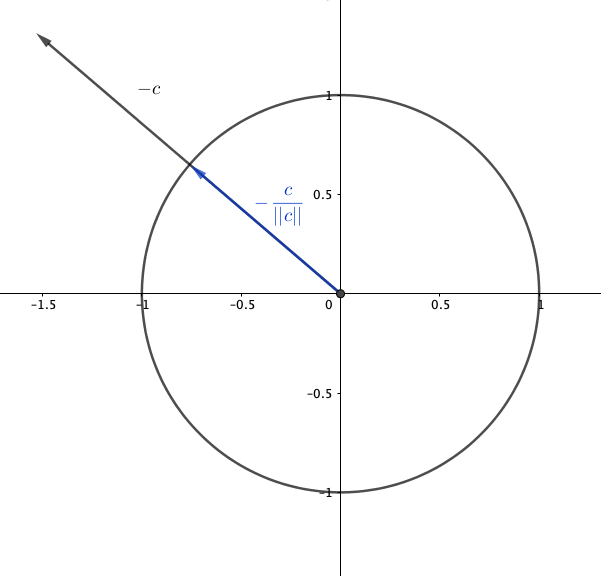
\includegraphics[width=.76\textwidth]{fig1.png}
        \end{center}
      \end{figure}
    \end{proof}
\vspace{.15in}


    \item[(b)] The necessary optimality conditions for this problem are addressed by Theorem 14.15 on page 504 of the textbook. Compute the Lagrangian 
    and state the first-order necessary conditions in detail. 
    \begin{proof}[Solution] Recall, as in the previous problem that the first-order optimality conditions for the method of Lagrange Multipliers come from 
      minimizing the Lagrangian, however in this case note that our constraints are nonlinear and we only have equality constraints. So we get
      \begin{equation*}
        L(x, \lambda) = f(x) - \lambda^Tg(x).
      \end{equation*}
      In the case of our problem, recall that the constraints must be of the form $g(x) = 0$ so the Lagrangian is given by, 
      \begin{equation*}
        L(x, \lambda) = c^Tx - \lambda^T(x^Tx - 1).
      \end{equation*}
      Since we are working with equality constraints, our first-order necessary conditions are given by $\nabla L(x_*, \lambda_*) = 0$, 
      \begin{equation*}
        \nabla_xL(x, \lambda) = c^T - 2\lambda x = 0.
      \end{equation*}
      \begin{equation*}
        \nabla_\lambda L(x, \lambda) = -x^Tx + 1 = 0.
      \end{equation*}
      Note that since we only have one constraint $\lambda$ is a scalar. 
    \end{proof}
    \vspace{.15in}


    \item[(c)] Solve the conditions in $(b)$ algebraically to confirm the solution in part $(a)$.
    How many points $(x_*, \nabla_*)$ are there which satisfy the first-order necessary conditions?
    \begin{proof}[Solution] With some algebra on $\nabla_xL(x, \lambda)$ we find that, 
      \begin{align*}
        c^T - 2\lambda x &= 0\\
        c^T &= 2\lambda x
      \end{align*}
      This implies that $||c|| = 2 |\lambda| ||x||$. But we know that $||x|| = x^Tx = 1$ and therefore $-||c|| = 2\lambda$ when $\lambda < 0$ and $||c|| = 2\lambda$ when $\lambda > 0$.
      Solving for $x$ we can divide through by $2\lambda$ since it's a scaler, and by substitution we get two solutions, 
      \begin{equation*}
        \pm\frac{c^T}{||c||} = x.
      \end{equation*}
      Solving for $\lambda$, we take $c^T = 2\lambda x$ applying $x^T$ to the right we get, $c^Tx^T = 2\lambda x^Tx = 2\lambda$. Substitution our solution for $x$ we get,
      \begin{equation*}
        \frac{c^Tx^T}{2} = \pm\frac{c^Tc}{2||c||} = \pm\frac{1}{2} = \lambda.  
      \end{equation*}
      Putting our solutions together we get that
      \begin{equation*}
        \left(-\frac{c^T}{||c||},-\frac{1}{2} \right),
      \end{equation*}
      \begin{equation*}
        \left(\frac{c^T}{||c||},\frac{1}{2} \right),
      \end{equation*}
      satisfy the first-order necessary conditions. 
    
    \end{proof}

  \end{enumerate}  
\end{exercise}
\vspace{.5in}



\begin{exercise}{P22} Consider the problem,
  \begin{align*}
    \text{minimize: } &f(x) = (x_1  - 1)^2 + (x_2 + 1)^2\\
    \text{subject to: } &x_1^2 + x_2^2 \leq 9\\
    &x_2 \geq 0
  \end{align*}
  \begin{enumerate}
    \item[(a)] Sketch the feasible set and explain informally, perhaps using contours of $f$, why 
    $x_* = (1,0)^T$ is the solution. \\
    \begin{proof}[Solution] Below is a graph of the feasible set with the contour lines of the objective function graphed on top. 
      We can see that in the area that defines the feasible set, the positive half circle we know that the direction of the $-\nabla f(x)$
      at any point is perpendicular to the contour lines. We also know that the direction of steepest descent is interior to the contour lines 
      since $f(x)$ is convex ($\nabla^2 f(x)$ is diagonal matrix with 2 on the diagonal but also a paraboloid that opens in the positive $z$ direction).
      
      \begin{figure}[H]
        \begin{center}
          \caption{Plotting the feasible set $S$ (positive half circle), and contours of $f(x)$.}
          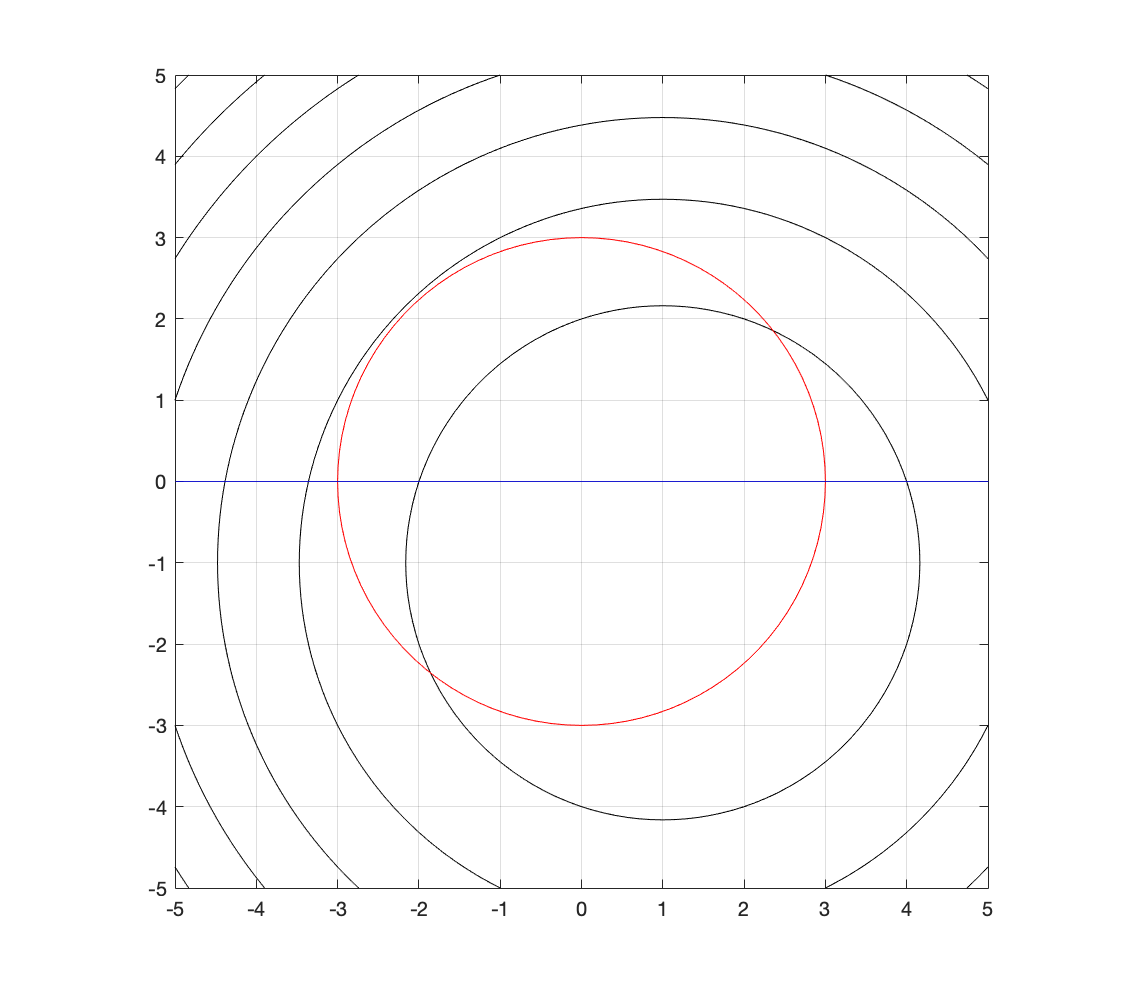
\includegraphics[width=.76\textwidth]{fig.png}
        \end{center}
      \end{figure}
    \vspace{.15in}

      Note that we have an unconstrained minimum at $(1, -1)$, and we can see that at point $(1,0)$ our descent direction is perpendicular to our active inequality constraint 
      $x_2 \geq 0$ in the direction outside the feasible set. So any feasible direction $p$ will result in $p\nabla f(x) < 0$ which implies that there are no feasible descent directions 
      at $(1,0)$ which means we are at a minimum, given our constraints. (word salad.)
    \end{proof}

    \item[(b)] Write the constraints in the form $g_i(x) \geq 0$. Compute the Lagrangian and it's gradient. 
    For each of the points $A = (0, 0)^T$, $B = (0, 3)^T$, and $C = (1, 0)^T$ compute the values of $\lambda_i$
    satisfying the zero gradient conditions. Address whether these points satisfy the first-order optimality conditions, 
    that is, whether they are candidates for a local minimizer. Show in particular that $C$ satisfies all the first-order conditions in
    Theorem 14.18. 
    \begin{proof}[Solution] Rewriting the constraints in the form of  $g_i(x) \geq 0$, we get, 
      \begin{equation*}
       g_1(x) =  -x_1^2 - x_2^2 + 9 \geq 0
      \end{equation*}
      \begin{equation*}
        g_2(x) = x_2 \geq 0
      \end{equation*}
      Recall that the Lagrangian will be of the form, 
      \begin{equation*}
        L(x, \lambda) = f(x) - \lambda^Tg(x) = f(x) - \begin{pmatrix}
          \lambda_1\\
          \lambda_2
        \end{pmatrix}
        \left(g_1(x), g_2(x)\right)
      \end{equation*}
      Then the gradient of the Lagrangian with respect to $x$ is, 
      \begin{equation*}
        \nabla_x L(x, \lambda) = \nabla f(x) - \nabla g(x)\lambda = \begin{pmatrix}
          2(x_1 - 1)\\
          2(x_2 + 1)
        \end{pmatrix}
         - 
         \begin{pmatrix}
          -2x_1 & -2x_2\\
          0 & 1
         \end{pmatrix}
         \begin{pmatrix}
          \lambda_1\\
          \lambda_2
         \end{pmatrix}
      \end{equation*}
      Solving the $\lambda_i$ values for $A = (0, 0)^T$. Note that only one constraint is active and our feasible set lives in $\RR^2$ so $A$ is regular. Since the $g_1(x)$ constraint is inactive by complementarity $(\lambda^Tg(x) = 0)$ we know that 
      $\lambda_1 = 0$ and plugging in our values we get the following system which has no solution, so we say that the first-order stationarity condition is not satisfied, 
      i.e $\nabla_x L(A, \lambda) \neq 0$. 
      \begin{equation*}
        \begin{pmatrix}
          0& 0\\
          0& 1
        \end{pmatrix}
        \begin{pmatrix}
          0\\
          \lambda_2
         \end{pmatrix}
          = 
          \begin{pmatrix}
            -2\\
            2
           \end{pmatrix}
      \end{equation*}
      Solving the $\lambda_i$ values for $B = (0, 3)^T$. Again note that since only one constraint is active $B$ is regular. Since the $g_2(x)$ constraint is inactive by complementarity we know that $\lambda_2 = 0$
      and plugging in our values we get the following system with no solution and again the first-order stationarity condition is not satisfied. 

      \begin{equation*}
        \begin{pmatrix}
          0& -6\\
          0& 1
        \end{pmatrix}
        \begin{pmatrix}
          \lambda_1\\
          0
         \end{pmatrix}
          = 
          \begin{pmatrix}
            -2\\
            8
           \end{pmatrix}
      \end{equation*}
      Solving the $\lambda_i$ values for $C = (1, 0)^T$. Note that $C$ is regular just like the other points. Since the $g_1(x)$ constraint is inactive by complementarity we know that 
      $\lambda_1 = 0$ and plugging in our values we get the following system which has a solution at $\lambda_c = (0, 2)^T$. 
      \begin{equation*}
        \begin{pmatrix}
          -2& 0\\
          0& 1
        \end{pmatrix}
        \begin{pmatrix}
          0\\
          \lambda_2
         \end{pmatrix}
          = 
          \begin{pmatrix}
            0\\
            2
           \end{pmatrix}
      \end{equation*}
      Therefore the \textbf{first-order stationarity} condition is satisfied, $\nabla_x L(C, \lambda_c) = 0$.\\


      Next we check for \textbf{primal feasibility} if $g(x_*) \geq 0$. Clearly $g(C) = (-1 + 9, 0)^T = (8, 0) \geq 0$ so $g(C) \geq 0$. \\


      Checking for \textbf{dual feasibility} if $\lambda_* \geq 0$. Since $\lambda_c = (0, 2)^T \geq 0$ we get $\lambda_c \geq 0$.\\


      Finally we check for \textbf{complementarity} if $\lambda_*^Tg(x_*) = 0$. Doing so we get $\lambda_c^Tg(C) = (0, 2)^T(8, 0) = 0$ so 
      $\lambda_c^Tg(x_c) = 0$. Point $C$ is the only candidate to be a local minimizer, we would proceed by checking the positive definiteness of 
      $Z(C)^T \nabla^2_{xx}L(C, \lambda_c) Z(C)$ where $Z(C)$ is a null space matrix of $\nabla g(x)$.   
    \end{proof}
  \end{enumerate}

\end{exercise}
\vspace{.5in}


\begin{exercise}{P23} Consider nonlinear optimization problems in $x \in \RR^n$ which have the standard-form linear constraints:
  \begin{align*}
    \text{minimize: } &f(x)\\
    \text{subject: } &Ax = b\\
    &x \geq 0
  \end{align*}
  Assume that there are $m$ scalar constraint equations and that $A$ has full row rank. Thus $A \in \RR^{mxn}$, $b \in \RR^m$ and $m \leq n$.

  We want to visualize the possible feasible sets for such problems. For $3D(n = 3)$ there are four nonempty, and bounded if $m > 0$, possibilities. 
  Sketch the four corresponding cartoons. These cartoons should have the same annotations as the $2D$ versions.\\
  \begin{proof}[Solution] In the $m = 0$ case, the feasible set is simply the whole first octant, because of the positivity constraints, 
    \begin{figure}[H]
      \begin{center}
        \caption{$m = 0$}
        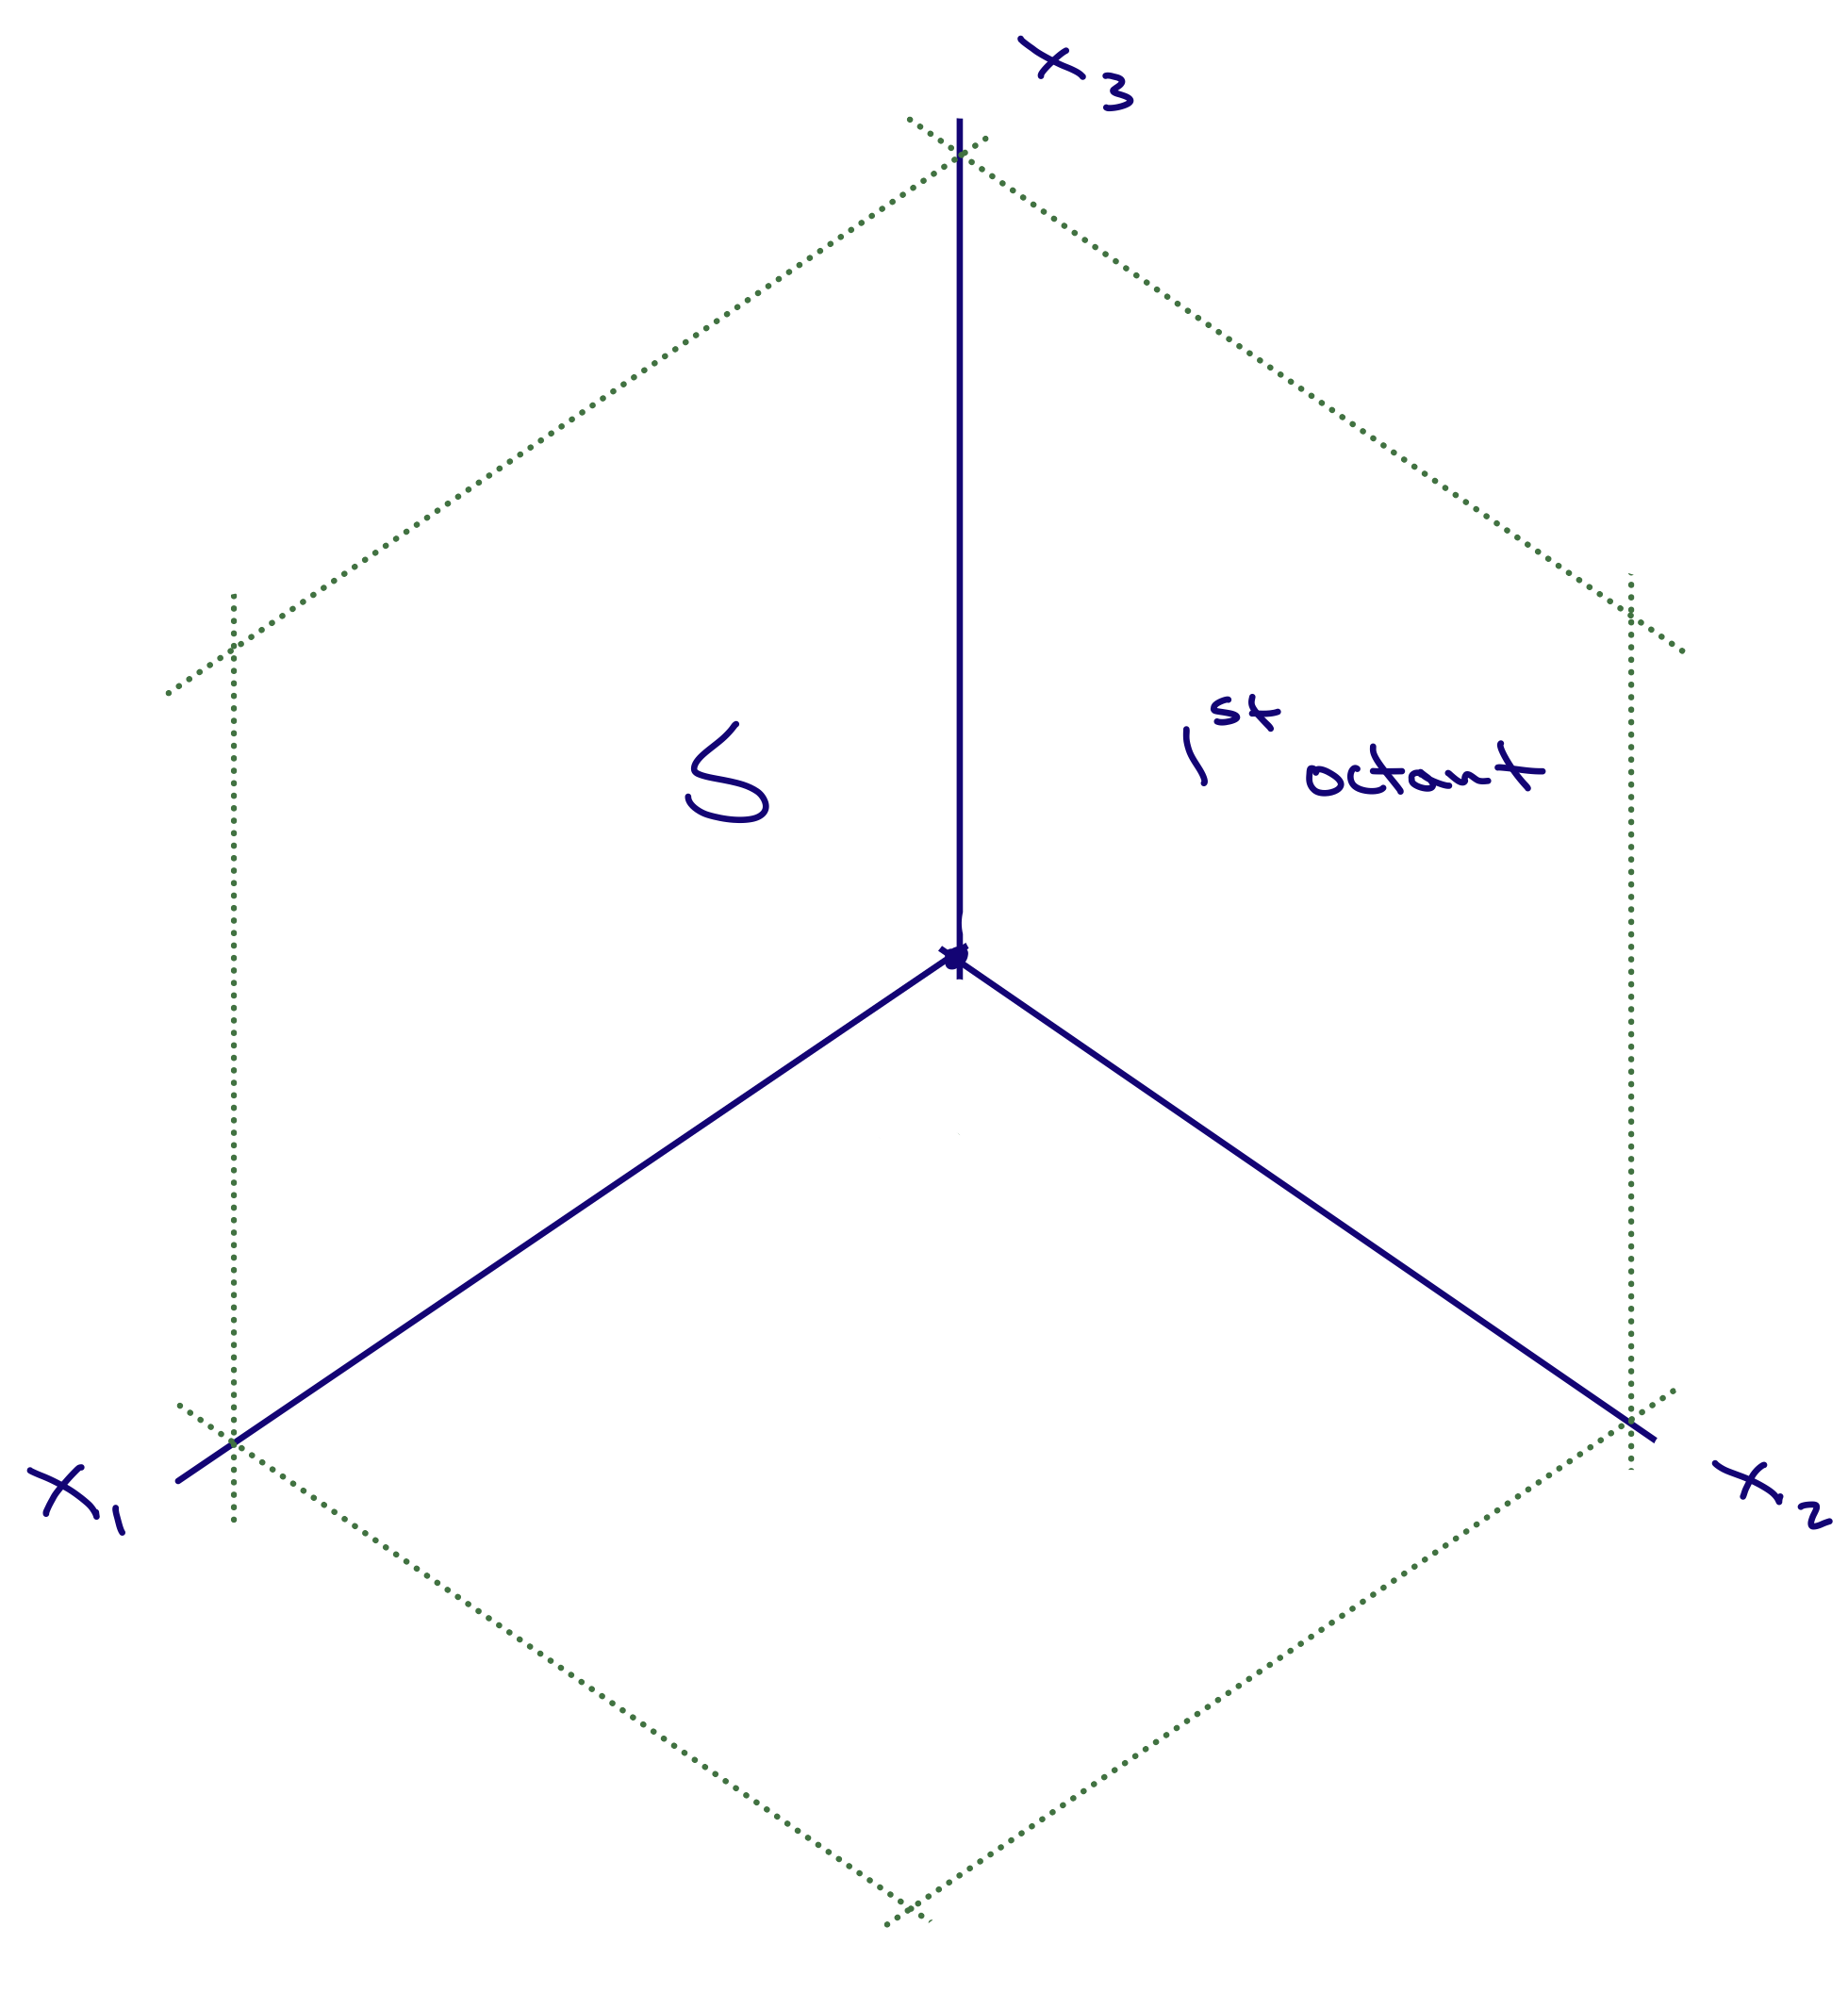
\includegraphics[width=.65\textwidth]{m0.png}
      \end{center}
    \end{figure}

    In the $m = 1$ case, the one linear constraint $a_1x + a_2y + a_3z = b_1$ defines a plane in $\RR^3$ with normal $n = (a_1, a_2, a_3)$. Assuming the feasible set is nonempty it would look like a triangular intersection of the plane inside the first octant. 
    \begin{figure}[H]
      \begin{center}
        \caption{$m = 1$}
        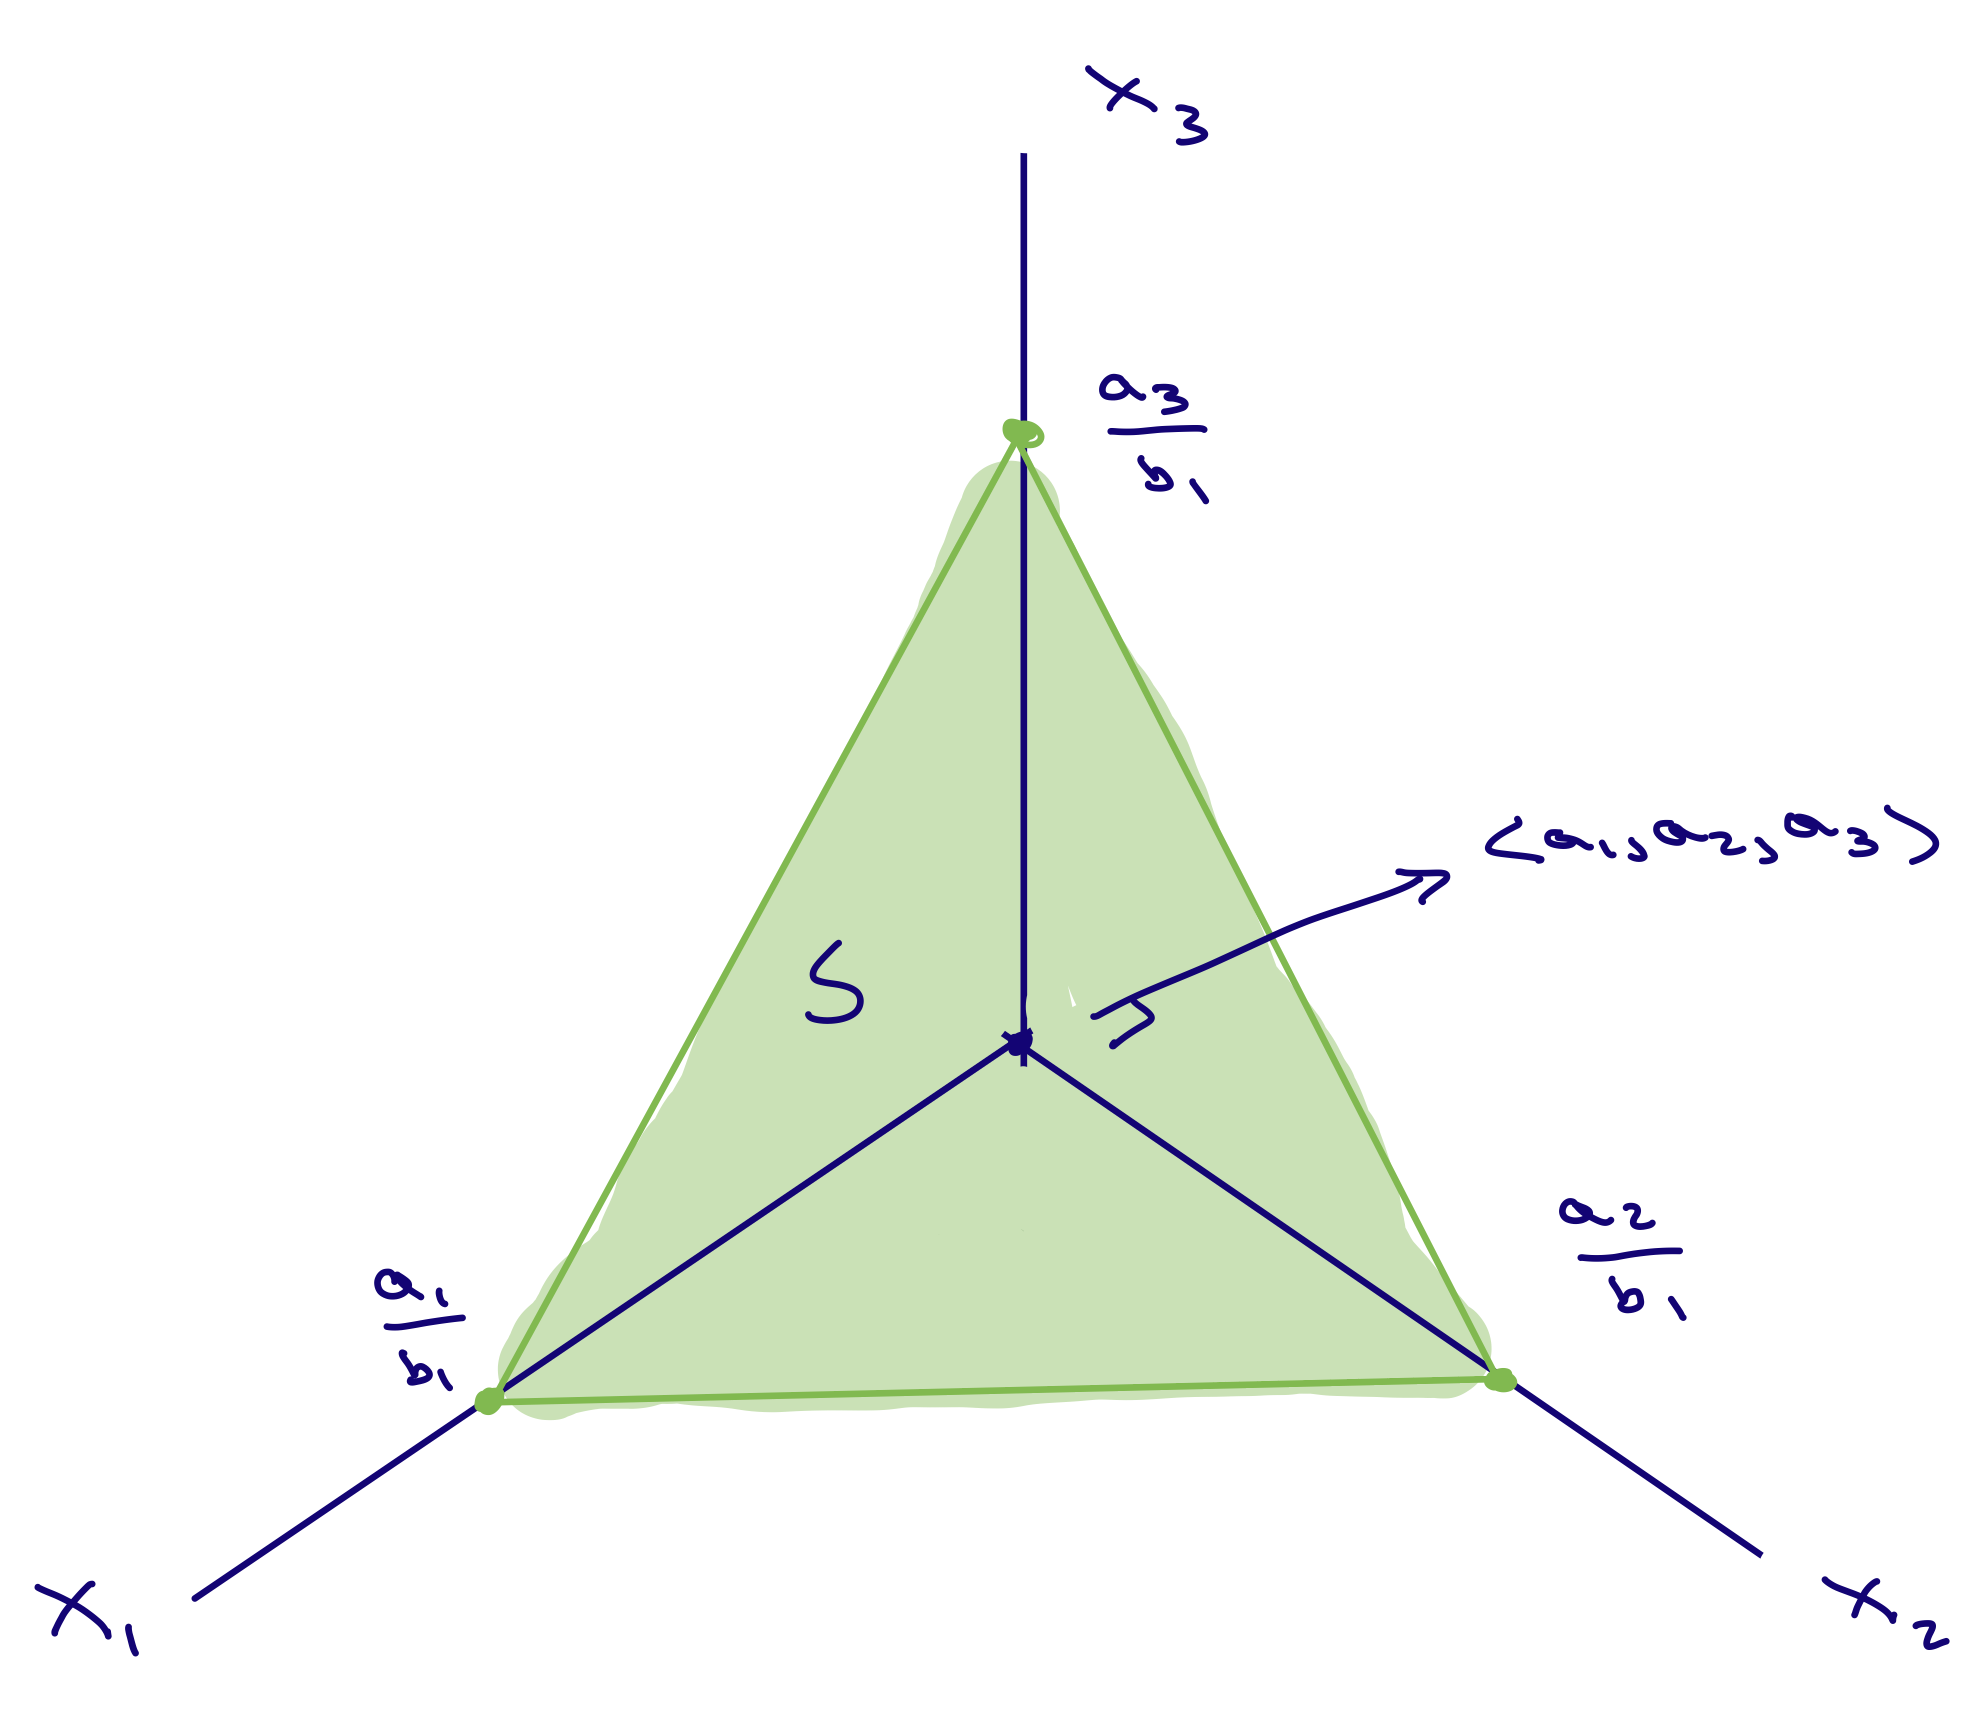
\includegraphics[width=.65\textwidth]{m1.png}
      \end{center}
    \end{figure}

    In the $m = 2$ case, the two linear constraints define two planes just like before. Since $A$ is full row rank we know that the normals of these planes do not point in the same direction
    and therefore they are not parallel. Again assuming the feasible set is nonempty the two planes must intersect at a line which also exists in the first octant. 
    \begin{figure}[H]
      \begin{center}
        \caption{$m = 2$}
        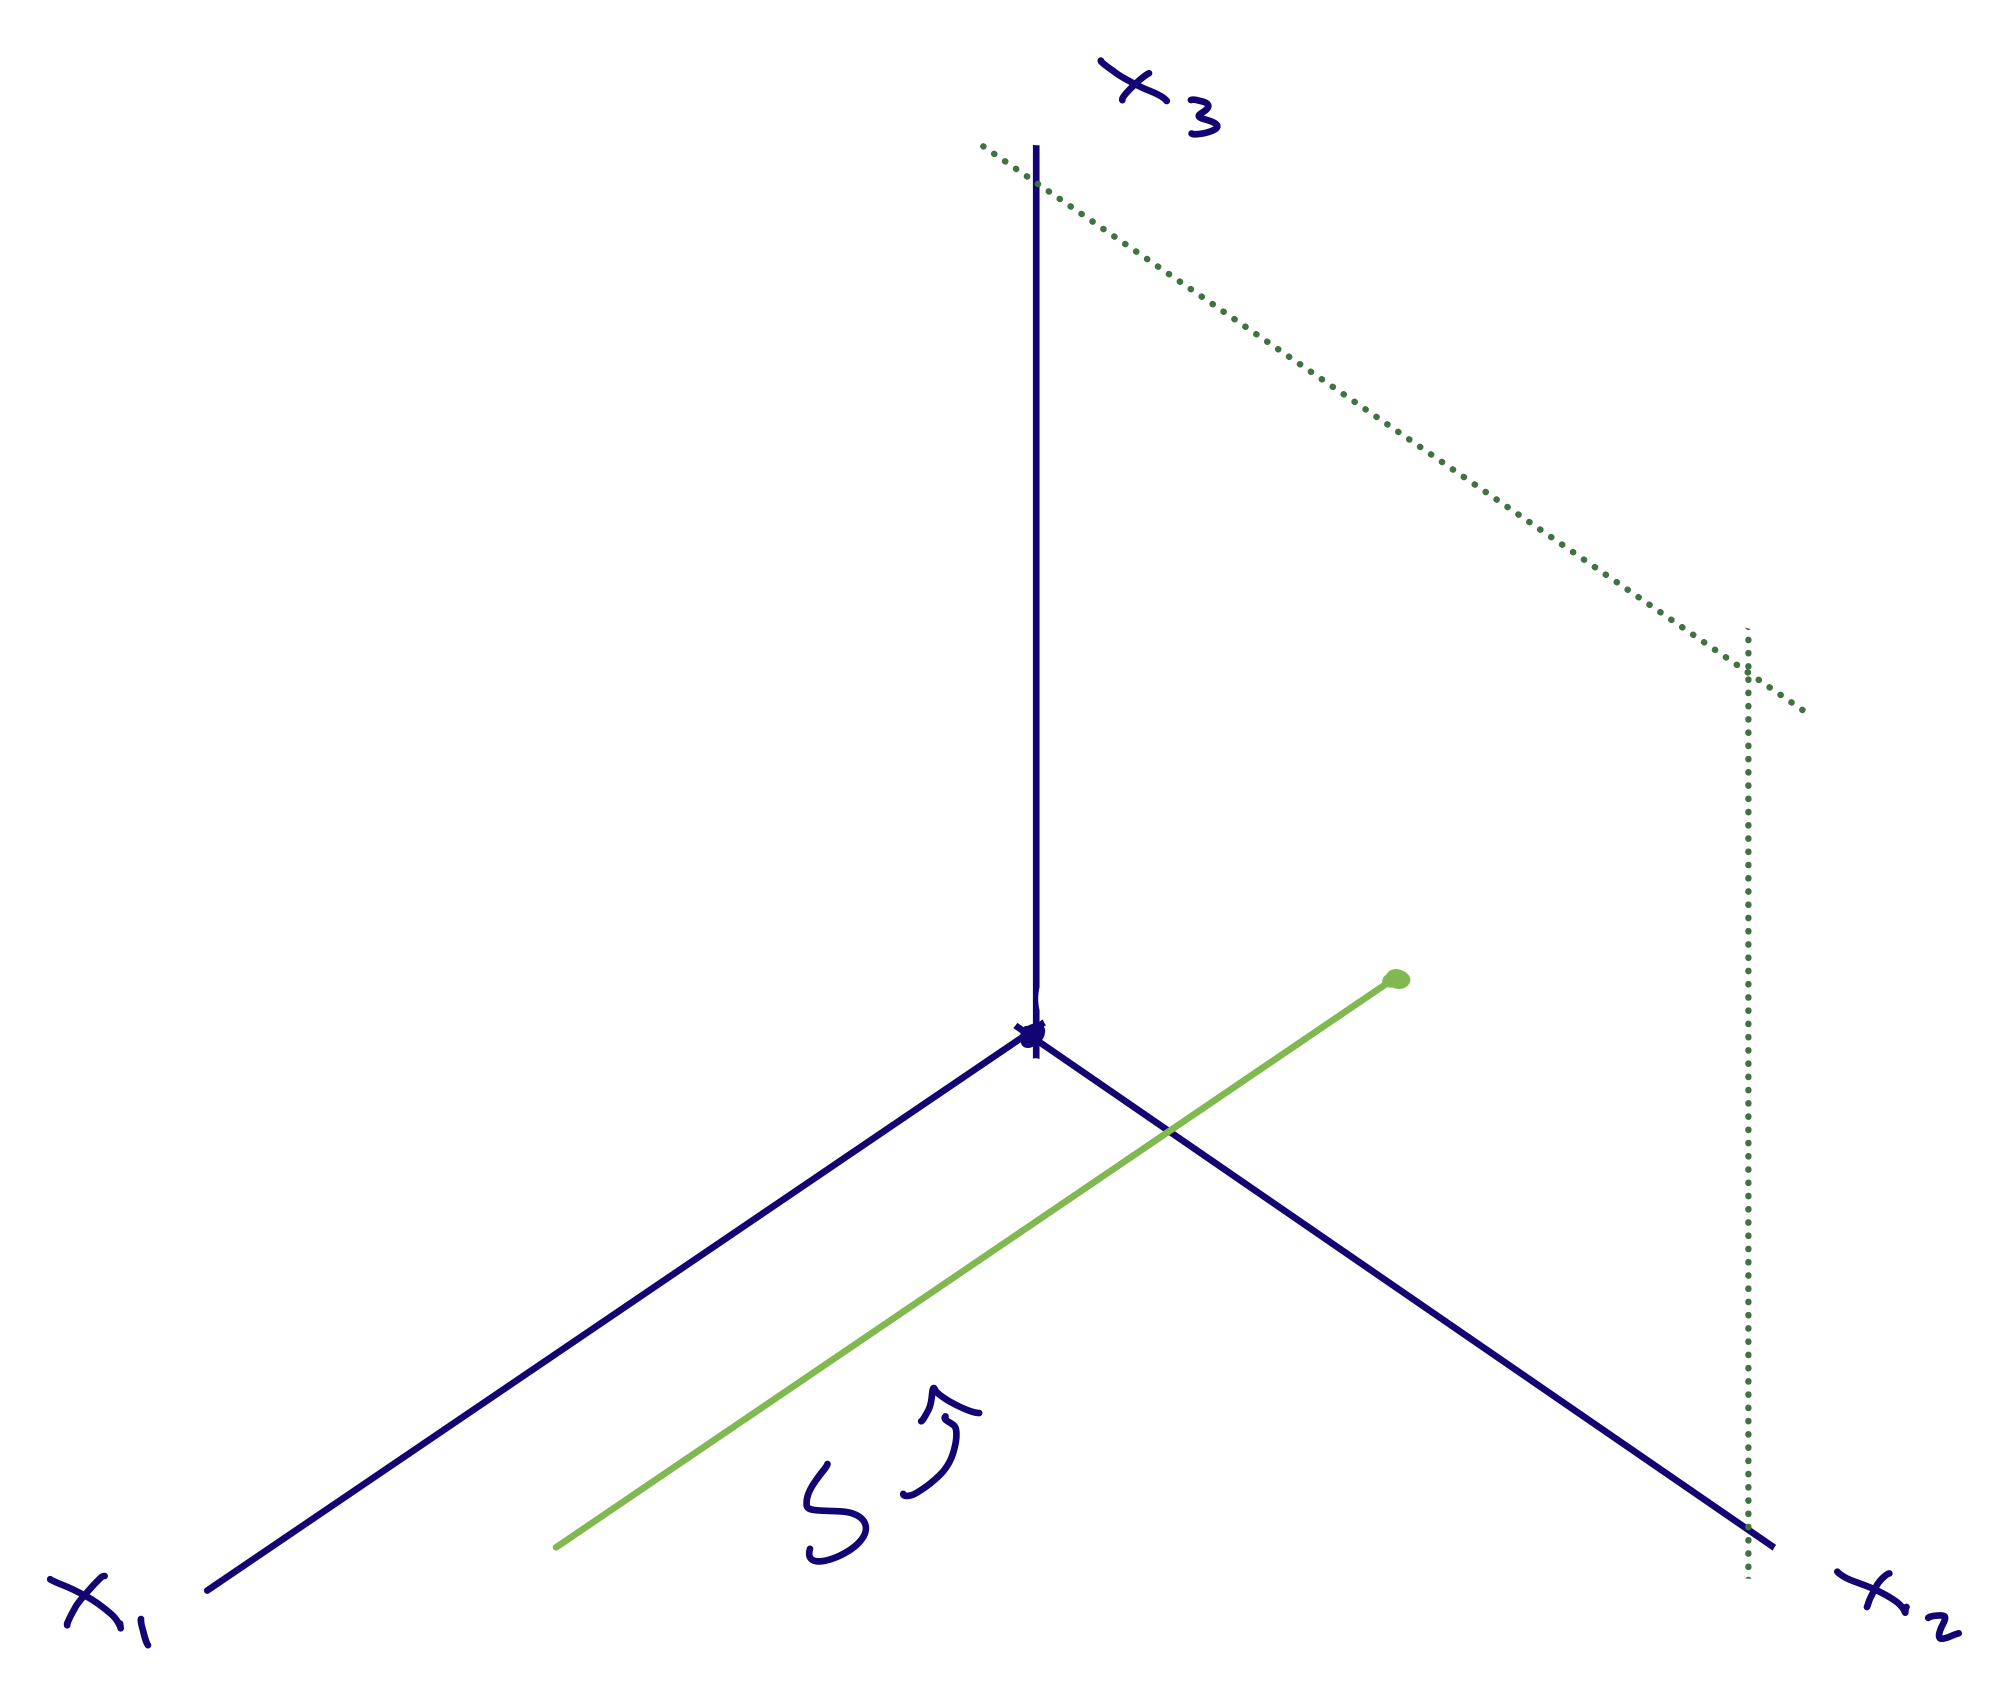
\includegraphics[width=.65\textwidth]{m2.png}
      \end{center}
    \end{figure}

    In the $m = 3$ case, simply note that $A$ must be invertible since $A$ is a square full row rank matrix. So there must be a solution to the system $Ax = b$, and assuming the feasible set 
    is nonempty this point must live in the first octant. 
    \begin{figure}[H]
      \begin{center}
        \caption{$m = 3$}
        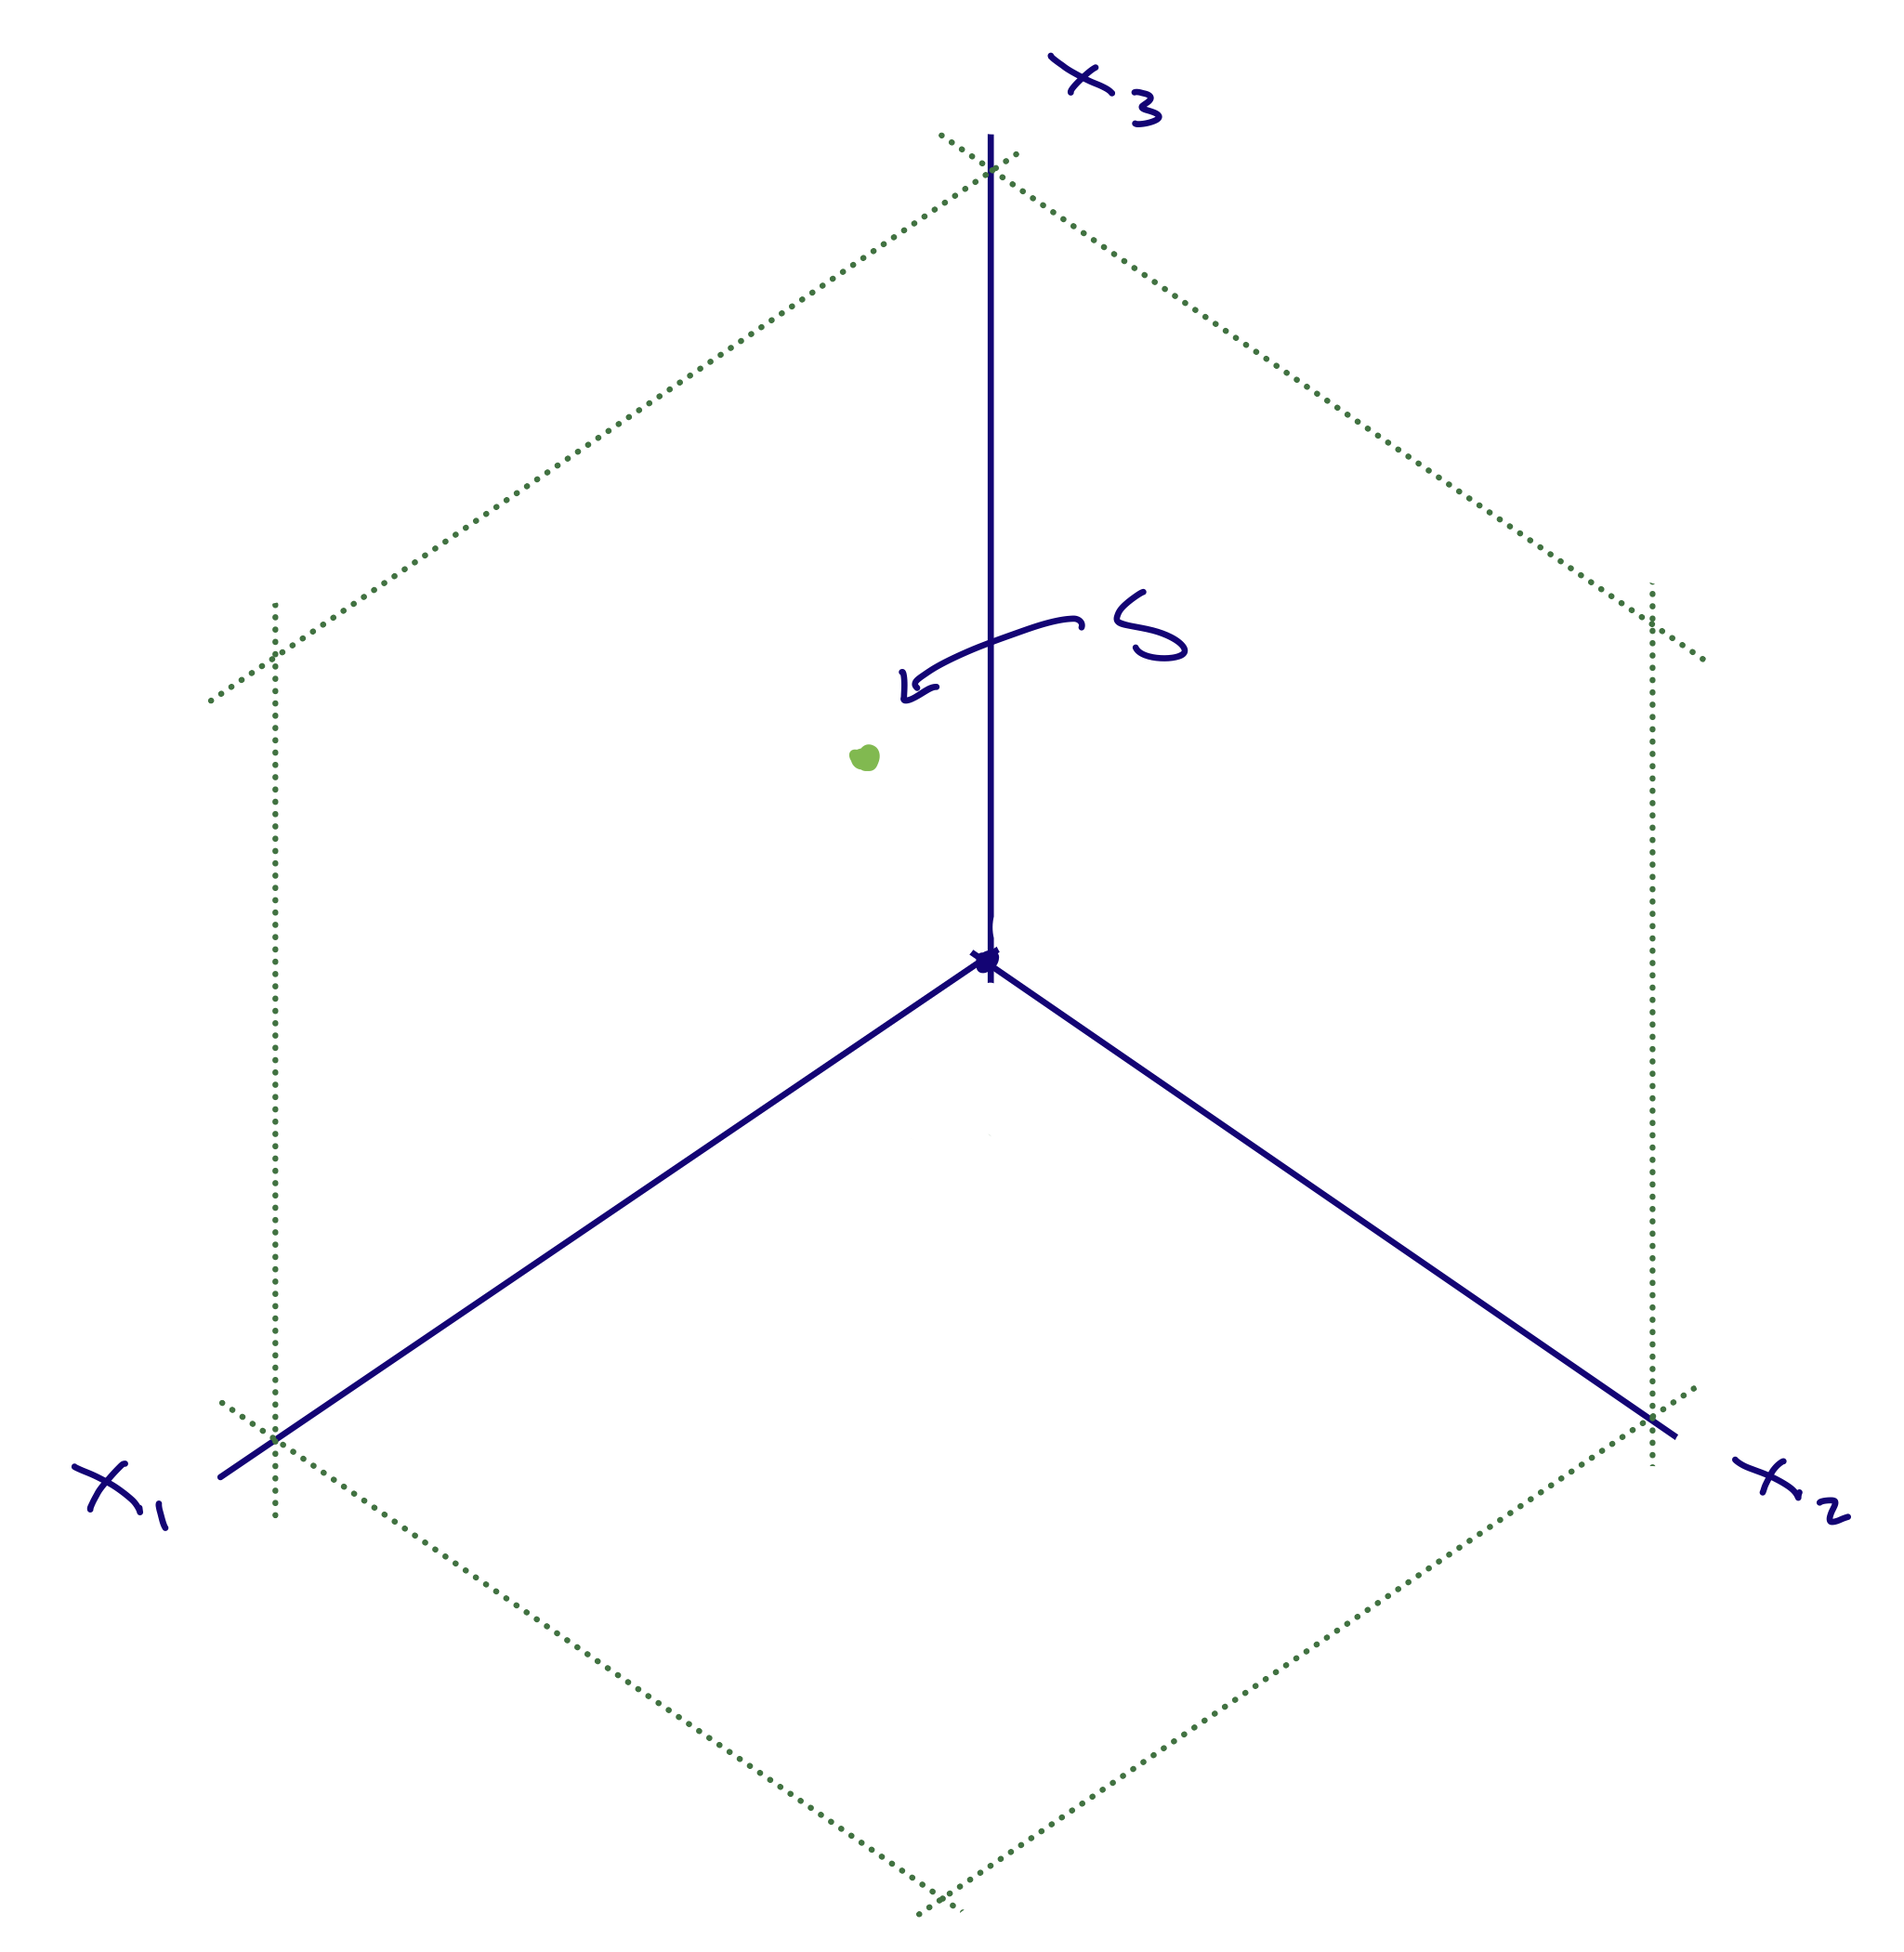
\includegraphics[width=.65\textwidth]{m3.png}
      \end{center}
    \end{figure}
    
  \end{proof}
\end{exercise}
\vspace{.5in}





\begin{exercise}{P24} Consider the general nonlinear constrained optimization problem over $x \in \RR^n$:
  \begin{align*}
    \text{minimize: } &f(x)\\
    \text{subject to: } g_i(x) &= 0, i = 1, \dots, l\\
    h_i(x) &\geq 0, j = 1, \dots, m
  \end{align*} 

  \begin{enumerate}
    \item[(a)] In section 14.5 the meaning of the phrase \emph{'$x_*$ is a regular point of the constraints'} is given
    state this definition precisely for the above problem. 
    \begin{proof}[Solution] First let $\hat{I}_x$ be the index of active constraints for point $x$. Let h'(x) = $\{h_j(x_*): i \in \hat{I}_{x_*}\}$.
      We say that $x_*$ is a \emph{regular point} of the constraints if the the block Jacobian matrix $[\nabla g(x); \nabla h'(x)]$ is full row rank.
    \end{proof}
  \vspace{.15in}

  \item[(b)] State the Lagrangian for this problem. 
    \begin{proof}[Solution] The Lagrangian for this problem is, 
      \begin{equation*}
        L(x, \mu, \lambda) = f(x) - \lambda^Tg(x) - \mu^Th(x).
      \end{equation*}
    \end{proof}
  \vspace{.15in}

  \item[(c)] Suppose $x_*$ is a local minimizer of the above problem which is also a regular point. 
  State the first-order necessary conditions for the above problem. 
  \begin{proof}[Solution] For $x_*$ to be a local minimizer it must satisfy the \textbf{stationarity} conditions, 
    \begin{equation*}
      \nabla_x L(x, \mu, \lambda) = \nabla f(x) - \nabla g(x)\lambda - \nabla h(x)\mu.
    \end{equation*} 
    Note that $x_*$ must also satisfy \textbf{primal feasibility},
    \begin{align*}
      h(x_*) &\geq 0,\\
      g(x_*) &= 0.
    \end{align*}
    Since the dual variables of the equality constraints are unconstrained, we must only check \textbf{dual feasibility}
    for the dual variables of the inequality constraints, 
    \begin{equation*}
      \mu \geq 0. 
    \end{equation*}
    As a consequence of strong duality $x_*$ must satisfy the \textbf{complementarity} condition, 
    \begin{equation*}
      \mu^Th(x) = 0.
    \end{equation*}

  \end{proof}


  \end{enumerate}
\end{exercise}
\vspace{.5in}





\end{document}




























